We present SeedProteo, a diffusion-based model for \textit{de novo} all-atom protein design. We demonstrate how to repurpose a cutting-edge folding architecture into a powerful generative design framework by effectively integrating self-conditioning features. Extensive benchmarks highlight the model's capabilities across two distinct tasks: in unconditional generation, SeedProteo exhibits superior length generalization and structural diversity, maintaining robustness for long sequences and complex topologies; in binder design, it achieves state-of-the-art performance among open-source methods, attaining the highest in-silico design success rates, structural diversity and novelty. Finally, we validate SeedProteo through wet-lab assays on two therapeutic targets, achieving hit rates of 70\%--80\% and picomolar-level binding affinities, establishing leading results. To facilitate community adoption, we provide public access to SeedProteo via a webserver (\url{https://seedfold.io/proteinDesign}).

\vspace{2mm}
\begin{center}
    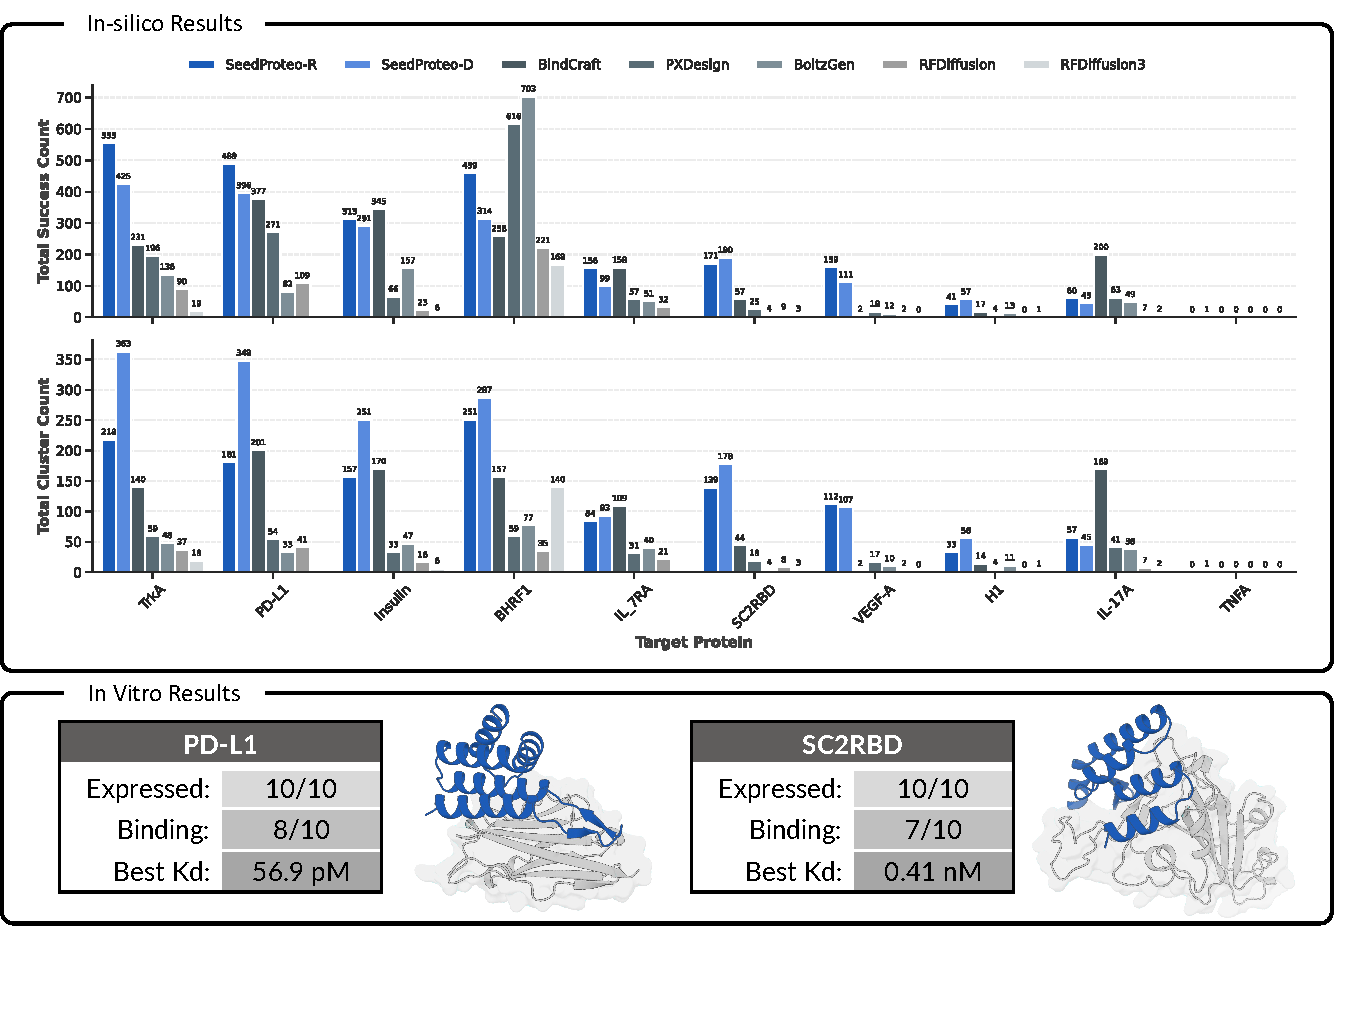
\includegraphics[width=0.9\linewidth]{figures/abstract_fig.pdf}
    \label{fig:front}
\end{center}

\vspace{-10mm}